\section{Purely Syntactic Translations}

\begin{itemize}
    \item 1-1 map between the rules
    \item Rules differ only by terminal symbols
    \item Rules with same nonterminals, in same order
\end{itemize}

\subsection{From translation grammar to ELL with write}
\textbf{Note}: $G_1$ must be ELL(k).

Just add write actions where needed in the ELL parser.

\subsection{From translation grammar to ELR with write}
Write actions only at reduction time, $G_t$ must be normalized in \emph{postfix normal form}.

Every rule of $G_2$ must be $A \rarr \gamma w$ where $\gamma\in V^*$ and $w \in \Delta^*$ ($\Delta$ is target terminal set). Introduce additional nonterminals replacing the non-suffix terminals. \textbf{Note}: this can lose ELR(1).

\subsection{2I-machine}

It gets 2 inputs, the source and target string and accepts if the second is the translation of the first. To accept both tapes must be scanned completely.

\subsection{IO-automation}

The second tape is the output and the machine computes the translation as a function of the source.

An IO-automation is deterministic if the automaton with only the numerators is deterministic.

\subsection{Sequential Transducer}

Variant of IO-automation that emits while executing transitions and eventually writing also when exiting ($\frac{\dashv}{s}$)

\begin{figure}[H]
    \centering
    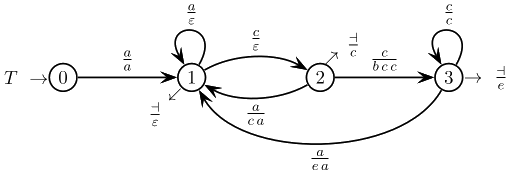
\includegraphics[width=0.9\linewidth]{syntax/sequential-transducer.png}
\end{figure}

\subsection{Rational Translation Expression}

A regular expression where the terminals are fractions, for example:
$R_\tau = \frac{(}{(} \left( \frac{a}{a} | \frac{(}{\epsilon} \left(\frac{a}{2a}\right)^+ \frac{)}{\epsilon} \right)^+ \frac{)}{)}$
